\documentclass[xcolor=table,dvipsnames]{beamer}

\usepackage{lscape, amsmath, amsfonts, amssymb, setspace, theorem, wrapfig, graphicx, float, multirow, subfig, color, rotating, multicol, datetime, natbib, venndiagram, pstricks, xkeyval, tikz, etoolbox, verbatim, pgf, tikz, pgfplots, mathrsfs, nth}

\usepackage{listings}
\usepackage{xcolor}
\usetikzlibrary{arrows}

\definecolor{codegreen}{rgb}{0,0.6,0}
\definecolor{codegreengray}{rgb}{0,0.4,0}
\definecolor{codegray}{rgb}{0.5,0.5,0.5}
\definecolor{codeblue}{rgb}{0.00,0,0.82}
\definecolor{backcolour}{rgb}{0.95,0.95,0.92}
\definecolor{jeopardy}{rgb}{.24,.47,.914}

\lstdefinestyle{mystyle}{
    backgroundcolor=\color{backcolour},   
    commentstyle=\color{codegreengray},
    numberstyle=\tiny\color{codegray},
    stringstyle=\color{codegreen},
    basicstyle=\ttfamily\footnotesize,
    breakatwhitespace=false,         
    breaklines=true,                 
    captionpos=b,                    
    keepspaces=true,                 
    numbers=left,                    
    numbersep=5pt,                  
    showspaces=false,                
    showstringspaces=false,
    showtabs=false,                  
    tabsize=2
}
 
\lstset{style=mystyle}

\title{GV300 - Quantitative Political Analysis}
\subtitle{University of Essex - Department of Government}
\date{Week 24 -- 9 March, 2020}				% or you can specify a date, just write it down instead of "\today"
\author{Lorenzo Crippa} 

\usetheme[progressbar=frametitle]{metropolis}
\usecolortheme{seahorse}						% try others: wolverine; crane...


\begin{document}

\begin{frame}[plain]
\begin{center}
\titlepage
\end{center}
\end{frame}

\begin{frame}{2020 Department of Government Student Conference}
\centering

\includegraphics[scale=0.35]{pictures/week24_conference.pdf} 
\end{frame}

\begin{frame}{Teaching evaluation. Be mindful of your unconscious biases!}
\centering
\begin{figure}
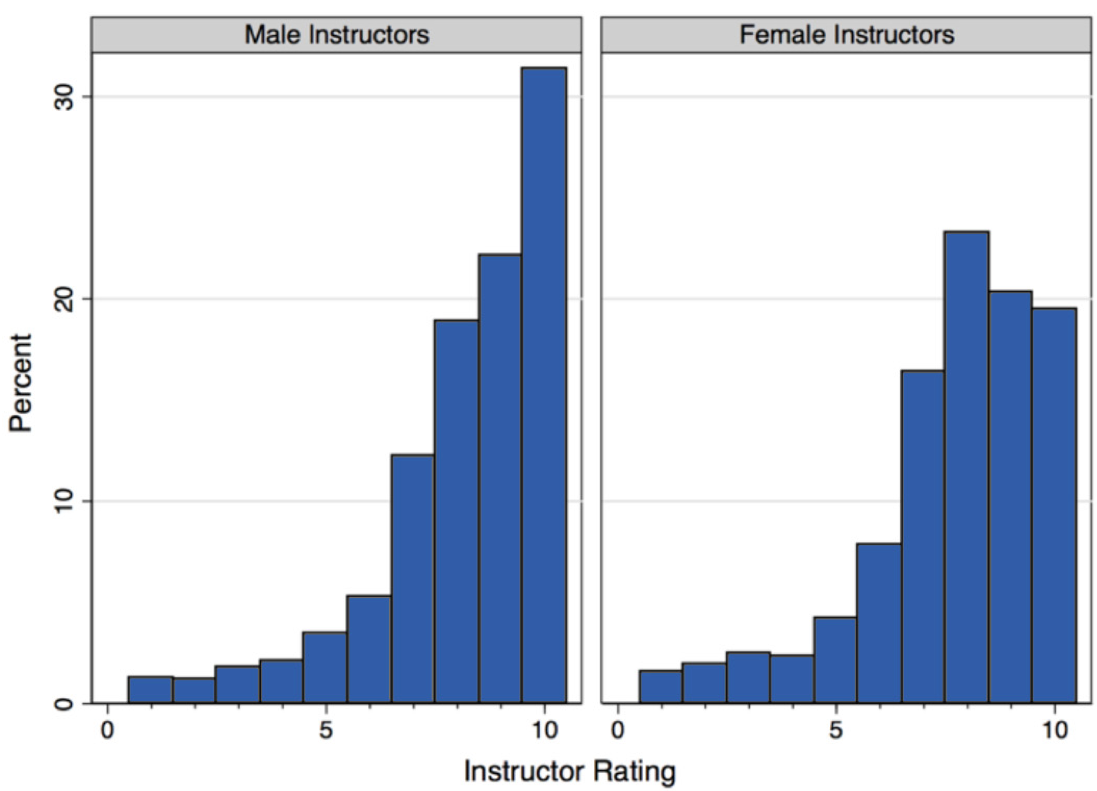
\includegraphics[scale=0.45]{pictures/week24_gender.png}
\caption{Source: Rivera and Tilcsik 2019}
\end{figure}
\end{frame}

\begin{frame}
\frametitle{Today's class}
\begin{enumerate}
\item Prep for exam: From Mac (or Linux) to PC
\item Correction of Problem Set 7
\item Maximum Likelihood Estimation
\end{enumerate}
\end{frame}

\section{Prep for exam: From Mac (or Linux) to PC}

\begin{frame}[fragile]
\frametitle{RStudio and Stata between Mac and PC}
\begin{itemize}
\item RStudio and Stata work identically on Mac (or Linux) and PC. \pause
\item You only need to change directory paths because Mac and Linux are UNIX systems, while Microsoft Windows is NT-based. \pause
\item These systems treat the / and \textbackslash characters differently, and we use these characters in setting up paths (for working directories, for saving graphs, for getting data\ldots) \pause
\item In a UNIX system (Mac or Linux) the / is different from a \textbackslash. you have: \texttt{/Users/Your\_{}name/Documents/your\_{}folder} \pause
\item In Microsoft Windows the / is identical to a \textbackslash. So you can have both: \texttt{C:/Users/Your\_{}name/Documents/your\_{}folder} and \texttt{C:\textbackslash{}Users\textbackslash{}Your\_{}name\textbackslash{}Documents\textbackslash{}your\_{}folder}
\end{itemize}
\end{frame}

\begin{frame}[fragile]
\frametitle{Dealing with two different systems}
If you need to work on both systems in R or Stata you can include both paths and comment out the one you don't need (depending on the machine you're working on). \pause My examples: \pause
\begin{lstlisting}[language=R]
# Lorenzo Macbook
setwd("/Users/Lorenzo/Dropbox/Shared_Essex/GTA/GV300")

# Lorenzo Essex
#setwd("C:/Users/lc19059/Dropbox/Shared_Essex/GTA/GV300")
\end{lstlisting}

\begin{lstlisting}
* Lorenzo Macbook
* cd "/Users/Lorenzo/Dropbox/Shared_Essex/GTA/GV300"

* Lorenzo Essex
cd "C:/Users/lc19059/Dropbox/Shared_Essex/GTA/GV300"
\end{lstlisting}
\end{frame}

\begin{frame}{Practical tips for the exam}
The exam is going to be on PCs. Follow these steps:
\begin{itemize}
\item Set the working directory as a FIRST thing you do \pause
\item Open the working directory in File Explorer \pause
\item Copy the path of your directory (the text in the bar that you have on top of the File Explorer) \pause
\item Paste it in RStudio or Stata under the respective ``change directory'' command \texttt{setwd()} or \texttt{cd} \pause
\item R works only if you turn each \textbackslash into a / while Stata works both ways \pause
\item In any case it's always better to change each \textbackslash into a /
\end{itemize}
\end{frame}

\section{Correction of Problem Set 7}

\begin{frame}[fragile]
\frametitle{Question 1 -- (a)}
Difference-in-differences: generate indicators for treatment-control groups and pre-post intervention. List countries in the two groups. \pause

\begin{lstlisting}[language = R]
data$treatment <- ifelse(data$yearJoinEU == 2004, 1, 0)
data$intervention <- ifelse(data$year >= 2004, 1, 0)
\end{lstlisting}
\begin{lstlisting}
gen treatment = 0 + (yearjoineu == 2004)
gen intervention = 0 + (year >= 2004)
\end{lstlisting} \pause
Countries in the treatment group: Czech Republic, Estonia, Hungary, Latvia, Lithuania, Poland, Slovak Republic, Slovenia. \pause

Countries in the control group: Albania, Armenia, Bulgaria, Croatia, Georgia, Kosovo,Macedonia, FYR Moldova, Montenegro, Serbia, Ukraine
\end{frame}

\begin{frame}
\frametitle{Question 1 -- (b)}
Compute the mean of \texttt{GDPPerCapita} for treatment and control group pre- and post-intervention. Plot those numbers. Compute the difference-in-differences from those numbers. \pause

The difference in differences is  $(15495.61-5306.678)-(4873.54-1574.61)=6890.301$
\end{frame}

\begin{frame}{Question 1 -- (b)}
\centering
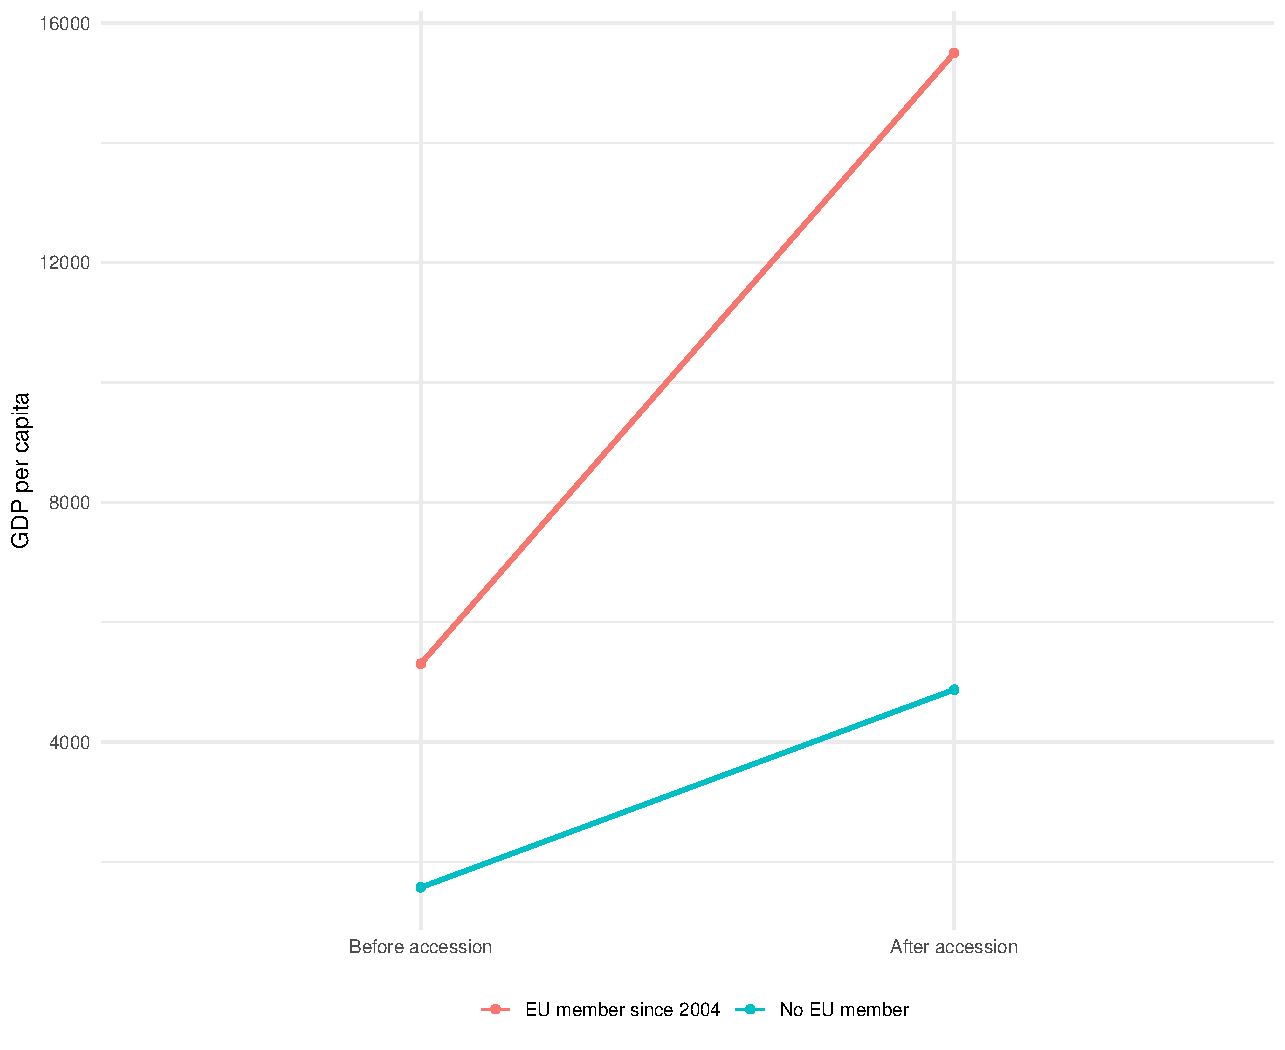
\includegraphics[scale=0.45]{pictures/week_24_Q1_b.pdf} 
\end{frame}


\begin{frame}{Question 1 -- (c)}
Plot the mean of \texttt{GDPPerCapita} for treatment and control group over \texttt{year}. Add a line indicating the intervention year. Add the counterfactual \texttt{GDPPerCapita}. Evaluate whether the common trend assumption is met pre-intervention. Are the parts of SUTVA met that are relevant to the goodness of the differences-in-differences estimator? Why or why not?
\end{frame}

\begin{frame}{Question 1 -- (c)}
\centering
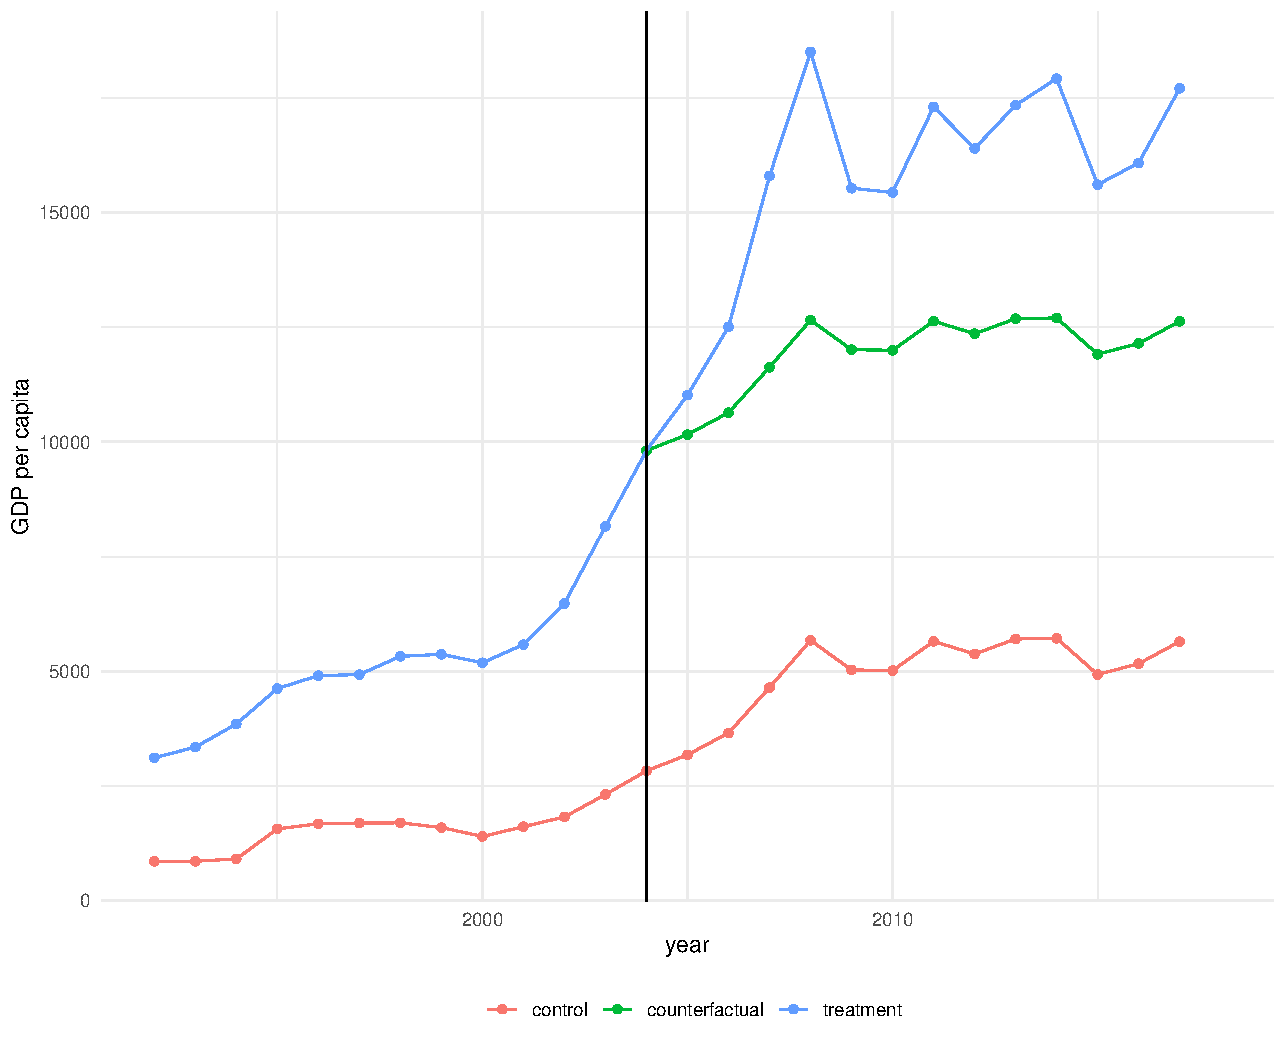
\includegraphics[scale=0.45]{pictures/week_24_Q1_c.pdf} 
\end{frame}

\begin{frame}{Question 1 -- (c): SUTVA}
It seems that GDP per capita is running in parallel in treatment and control group. \pause SUTVA for DiD requires: \pause
\begin{enumerate}
\item stability in composition of treatment and control group \pause
\item no spill-over effects
\end{enumerate} \pause
\begin{itemize}
\item Treatment group is constant: no country that joined the EU in 2004 left the EU until the end of the data set. \pause
\item Some countries in the control group joined the EU later which may bias our estimate of the causal effect of joining the EU. \pause
\item Spill-overs: it certainly may be that a rising GDP per capita thanks to joining the EU in, say, Slovenia may have affected the GDP per capita in neighbouring Croatia. \pause
\end{itemize} 

Hence, SUTVA may be violated
\end{frame}

\begin{frame}{Question 1 -- (d), (e) and (f)}
\begin{itemize}
\item[(d)] Run a regression to compute the differences-in-differences estimator. Report and interpret the result. Speak to the three relevant coefficients.
\item[(e)] Improve your regression in (d) by computing clustered standard errors.
\item[(f)] Improve your estimate of the causal effect of joining the EU in (e) by including one relevant country-level covariate into the regression. Report and interpret your result. Was your estimate in (e) an over- or underestimate of the causal effect? Speculate why failing to include this covariate led to bias in your estimate in (e).
\end{itemize}
\end{frame}

\begin{frame}{Question 1 -- (d), (e) and (f)}
\begin{table}
\begin{center}
\resizebox{100mm}{40mm}{
\begin{tabular}{l c c c c }
\hline
 & (d) & (e) & (f) & (f) \\
\hline
(Intercept)            & $1574.91^{***}$ & $1574.91^{***}$ & $-497.75$       & $6153.33^{***}$ \\
                       & $(299.71)$      & $(136.46)$      & $(314.89)$      & $(588.39)$      \\
intervention           & $3298.63^{***}$ & $3298.63^{***}$ & $2950.32^{***}$ & $3361.34^{***}$ \\
                       & $(390.18)$      & $(286.10)$      & $(297.74)$      & $(225.31)$      \\
treatment              & $3731.77^{***}$ & $3731.77^{***}$ & $2961.21^{***}$ & $241.61$        \\
                       & $(451.94)$      & $(315.27)$      & $(349.38)$      & $(547.94)$      \\
intervention:treatment & $6890.30^{***}$ & $6890.30^{***}$ & $5751.81^{***}$ & $6827.59^{***}$ \\
                       & $(593.70)$      & $(575.16)$      & $(608.09)$      & $(547.98)$      \\
exportsShareGDP        &                 &                 & $64.37^{***}$   &                 \\
                       &                 &                 & $(9.00)$        &                 \\
yearJoinEU             &                 &                 &                 & $-0.54^{***}$   \\
                       &                 &                 &                 & $(0.06)$        \\
\hline
R$^2$                  & 0.74            & 0.74            & 0.76            & 0.78            \\
Adj. R$^2$             & 0.73            & 0.73            & 0.75            & 0.78            \\
Num. obs.              & 457             & 457             & 451             & 457             \\
\hline
\multicolumn{5}{l}{\scriptsize{$^{***}p<0.01$, $^{**}p<0.05$, $^*p<0.1$}}
\end{tabular}
}
\end{center}
\end{table}
\end{frame}

\begin{frame}{Question 2 -- (a)}
Panel data exercise. Provide summary statistics and plots of the 6 variables in the data set that are not the panel identifiers year and state.
Plot \texttt{FTM} by state over time. 
\end{frame}

\begin{frame}{Question 2 -- (a)}
Summary statistics (pooled):
\begin{table}[!htbp] \centering 
\resizebox{100mm}{20mm}{
\begin{tabular}{@{\extracolsep{5pt}}lccccccc} 
\\[-1.8ex]\hline 
\hline \\[-1.8ex] 
Statistic & \multicolumn{1}{c}{N} & \multicolumn{1}{c}{Mean} & \multicolumn{1}{c}{St. Dev.} & \multicolumn{1}{c}{Min} & \multicolumn{1}{c}{Pctl(25)} & \multicolumn{1}{c}{Pctl(75)} & \multicolumn{1}{c}{Max} \\ 
\hline \\[-1.8ex] 
\texttt{FTM} & 201 & 58.249 & 9.516 & 26.296 & 53.364 & 63.511 & 91.833 \\ 
\texttt{white} & 261 & 0.809 & 0.162 & 0 & 0.7 & 0.9 & 1 \\ 
\texttt{poor} & 261 & 0.181 & 0.117 & 0.000 & 0.109 & 0.227 & 0.692 \\ 
\texttt{turnout} & 260 & 1.654 & 0.166 & 1.000 & 1.559 & 1.779 & 2.000 \\ 
\texttt{voteDem} & 261 & 0.164 & 0.171 & 0.000 & 0.000 & 0.295 & 0.667 \\ 
\texttt{dem} & 261 & 0.282 & 0.195 & 0.000 & 0.000 & 0.417 & 0.737 \\ 
\hline \\[-1.8ex] 
\end{tabular} 
}
\end{table}
\end{frame}

\begin{frame}{Question 2 -- (a)}
\centering
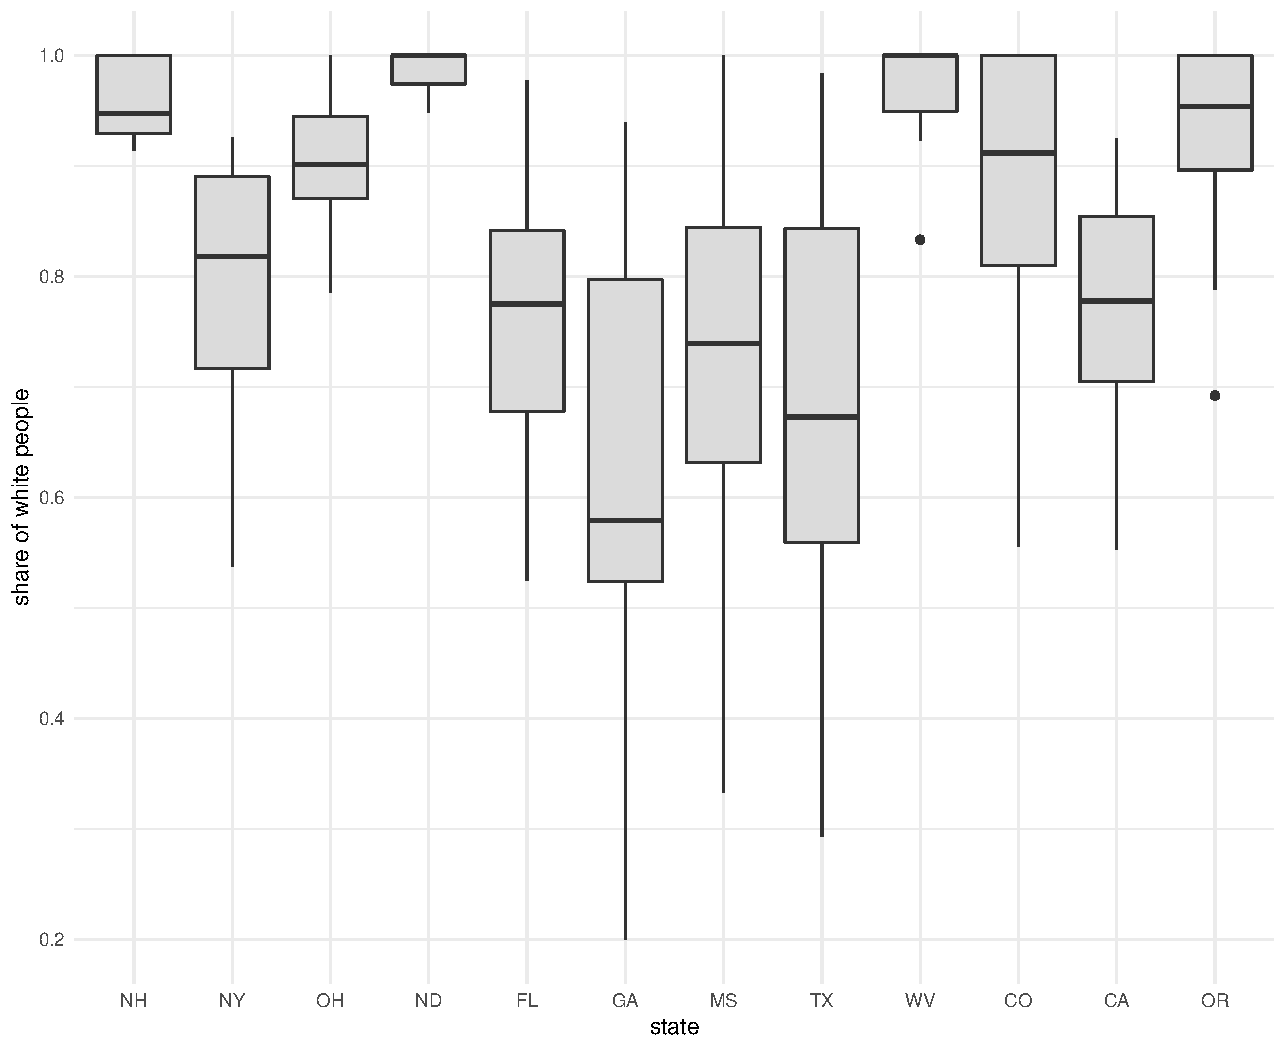
\includegraphics[scale=0.45]{pictures/week_24_Q2_a1.pdf} 
\end{frame}

\begin{frame}{Question 2 -- (a)}
\centering
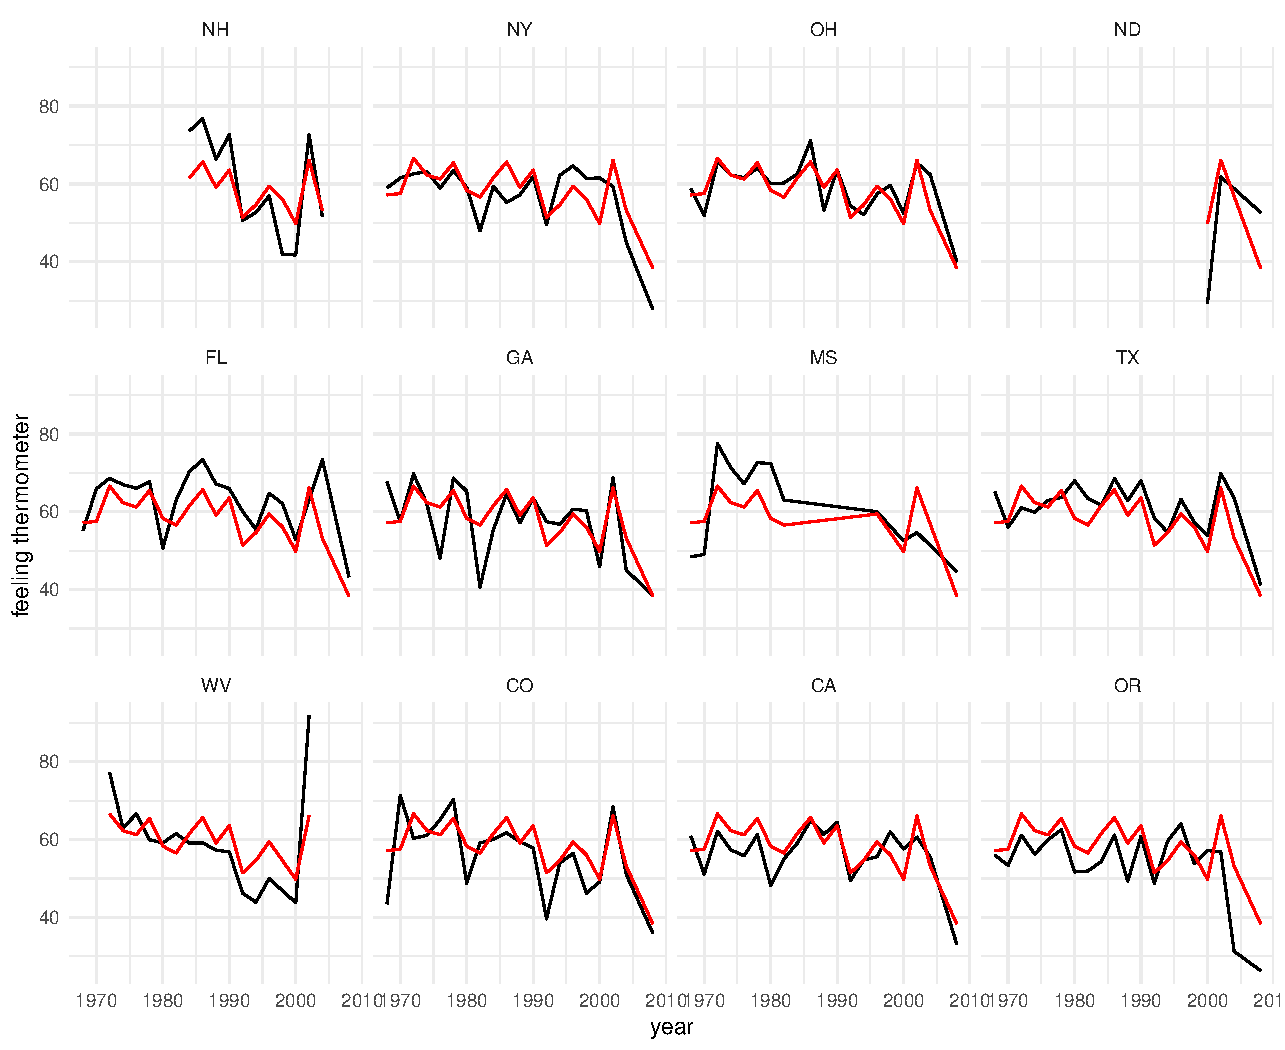
\includegraphics[scale=0.45]{pictures/week_24_Q2_a2.pdf} 
\end{frame}

\begin{frame}[fragile]
\frametitle{Question 2 -- (b)}
Get overall, within, and between variation (standard deviation) of the variables in the data set from R or Stata. \pause

\begin{verbatim}
overall.variation
    year      FTM     white      poor   
15.66012 9.516032 0.1615002 0.1174961

within.variation
var.year  var.FTM var.white  var.poor
15.06844 9.070157 0.1257591 0.1014254

between.variation
year_g.mean FTM_g.mean white_g.mean poor_g.mean
7.81        3.98       0.115        0.0725          
\end{verbatim}
\end{frame}

\begin{frame}{Question 2 -- (c), (d), (e), (f), (g)}
\begin{itemize}
\item[(c)] Run a pooled OLS regression of \texttt{FTM} on \texttt{white}, \texttt{poor}, \texttt{dem}, and \texttt{turnout}. Explain why the estimated coefficients and standard errors may be biased.
\item[(d)]  Re-run the regression above but allow errors to be clustered by \texttt{state}. How are the estimation results different? Explain why they are different.\\
\item[(e)] Re-run the regression above but include dummies for each state. How are the estimation results different? Explain why they are different.\\ 
\item[(f)] Re-run the regression above but use the fixed effects estimator (or within estimator). 
\item[(g)]  Re-run the regression above but use the random effects estimator. 
\end{itemize}
\end{frame}

\begin{frame}{Question 2 -- (c), (d), (e), (f), (g)}
\begin{table}
\begin{center}
\resizebox{100mm}{40mm}{
\begin{tabular}{l c c c c c }
\hline
 & (c) & (d) & (e) & (f) & (g) \\
\hline
(Intercept) & $83.91^{***}$  & $83.91^{***}$  & $50.52^{***}$  &                & $58.84^{***}$  \\
            & $(8.24)$       & $(11.07)$      & $(7.86)$       &                & $(5.87)$       \\
white       & $8.30^{**}$    & $8.30^{*}$     & $12.04^{*}$    & $12.04^{*}$    & $1.37$         \\
            & $(4.18)$       & $(4.47)$       & $(6.42)$       & $(7.28)$       & $(4.75)$       \\
poor        & $-5.66$        & $-5.66$        & $-1.83$        & $-1.83$        & $3.33$         \\
            & $(6.94)$       & $(10.35)$      & $(7.87)$       & $(10.42)$      & $(9.14)$       \\
dem         & $2.35$         & $2.35$         & $5.46$         & $5.46$         & $5.82^{*}$     \\
            & $(5.05)$       & $(4.48)$       & $(5.15)$       & $(3.55)$       & $(3.36)$       \\
turnout     & $-19.35^{***}$ & $-19.35^{***}$ &                &                &                \\
            & $(4.32)$       & $(4.59)$       &                &                &                \\
voteDem     &                &                & $-23.42^{***}$ & $-23.42^{***}$ & $-27.66^{***}$ \\
            &                &                & $(4.03)$       & $(3.00)$       & $(3.09)$       \\
\hline
R$^2$       & 0.10           & 0.10           & 0.29           & 0.22           & 0.22           \\
Adj. R$^2$  & 0.08           & 0.08           & 0.23           & 0.16           & 0.20           \\
Num. obs.   & 201            & 201            & 201            & 201            & 201            \\
\hline
\multicolumn{6}{l}{\scriptsize{$^{***}p<0.01$, $^{**}p<0.05$, $^*p<0.1$}}
\end{tabular}
}
\end{center}
\end{table}
\end{frame}

\begin{frame}[fragile]
\frametitle{Question 2 -- (h)}
Run the Hausman test and determine whether the fixed effects or the random effects model is more appropriate for the data at hand. \pause
\begin{verbatim}
     Hausman Test
data:  FTM ~ voteDem + dem + poor + white
chisq = 10.135, df = 4, p-value = 0.03822
alternative hypothesis: one model is inconsistent
\end{verbatim} \pause
\begin{itemize}
\item We reject the null, thus we should use a FE model. \pause 
\item \textbf{Yet} a Hausman test only cares about the precision of the estimate, and it is not everything we need to consider \pause
\item In this case we know we have lots of within and not so much between variation: a RE model still makes sense \pause
\item In these cases you can estimate both and hope to get similar results
\end{itemize}
\end{frame}

\section{Maximum Likelihood Estimation}

\begin{frame}{Introduction to MLE}
What is MLE? 
\begin{enumerate}
\item It's an estimation technique (we use it to estimate parameters, as in the LS framework) \pause
\item It is a statistical theory of inference \pause
\begin{itemize}
\item In probability theory we ask $p(y,\mathbf{X}|\theta)$ \pause
\item Yet in reality we start from our data $(y, \mathbf{X})$ and we want to find out what the parameters are! \pause
\item We want to find out the \textbf{likelihood} that the parameter is one that we estimate, given the data that we have. \pause
\item We are asking the same question, only starting from a different starting point: $p(y,\mathbf{X}|\theta)=\mathcal{L}(\theta|y,\mathbf{X})$ \pause
\item To perform MLE you need to have some prior idea of what functional form the distribution of your dependent variable can follow
\end{itemize}
\end{enumerate}
\end{frame}

\begin{frame}{Four steps to MLE}
\begin{enumerate}
\item Formulate the probability density function (PDF) of your $y$ \pause
\item Express the joint distribution of the observations with the PDF chosen and turn likelihoods into probabilities. Express the joint likelihood $\mathcal{L}$ as a log. (Assume i.i.d. observations): \pause
\end{enumerate}
$$ \mathcal{L} = \prod_{i=1}^{N}\mathcal{L}_i(\theta|y_i,\mathbf{X_i})= \prod_{i=1}^{N}p_i(y_i,\mathbf{X_i}|\theta) \rightarrow log\mathcal{L}= \sum_{i=1}^{N} log[p_i(y_i,\mathbf{X_i}|\theta)]$$ \pause
\begin{enumerate}
\item[3.] Take the first derivative of $log\mathcal{L}$ and set to 0 (first order condition) to find a maximum \pause $\frac{\partial log\mathcal{L}}{\partial \theta}=0$\pause
\item[4.] Take the second derivative and \textbf{verify} that it is smaller than 0 (second order condition) to verify it's a maximum (not a minimum) \pause $\frac{\partial^2 log\mathcal{L}}{\partial \theta}<0$
\end{enumerate}
\end{frame}

\begin{frame}{Log-likelihood function of a binomial distribution}
\centering
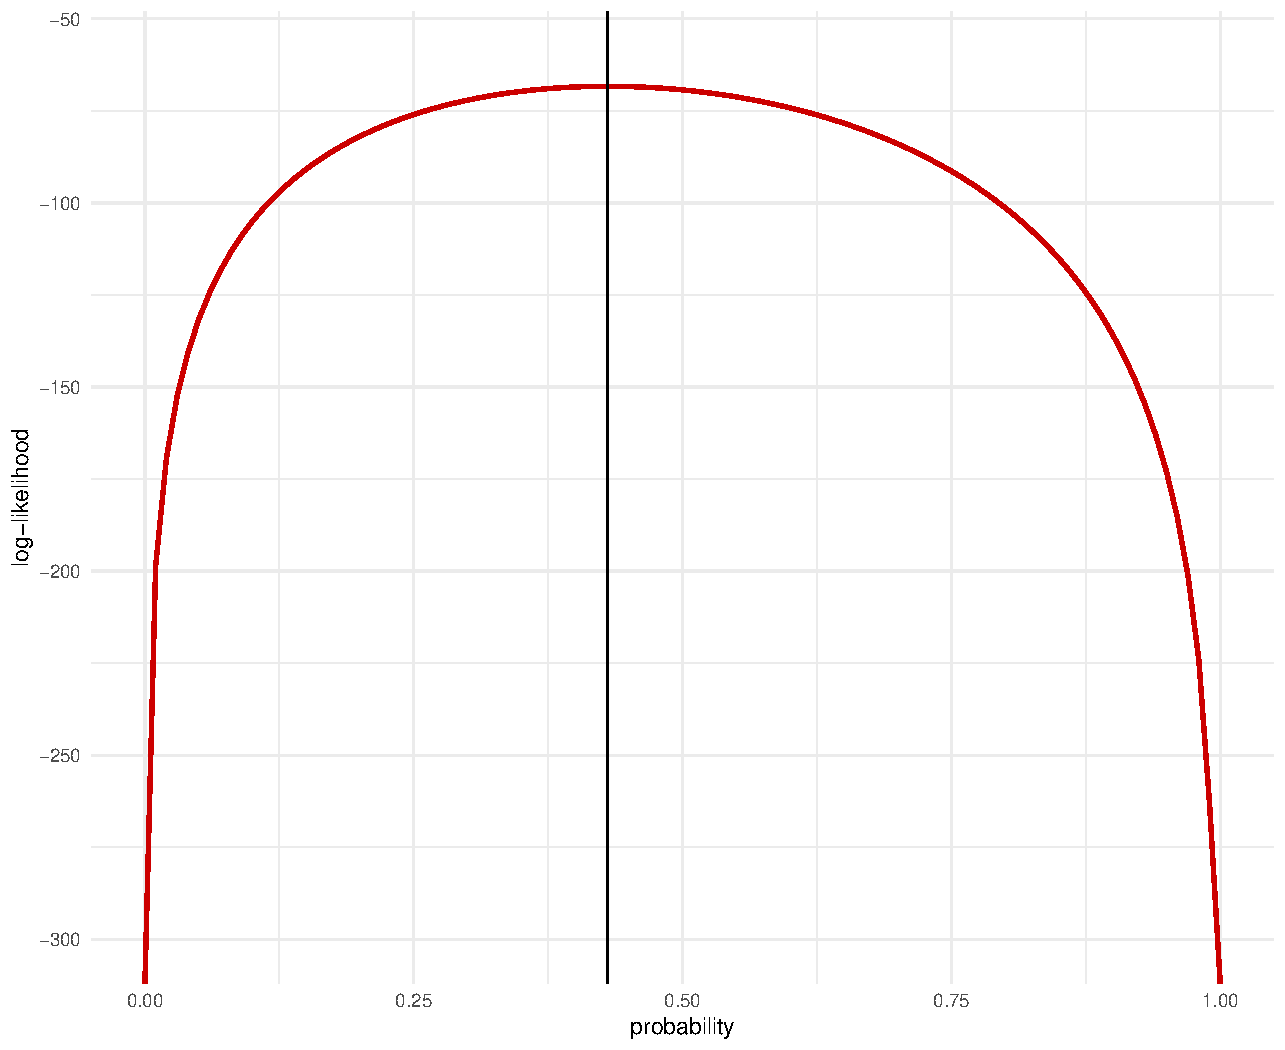
\includegraphics[scale=0.45]{pictures/week_24_ll_binomial.pdf} 
\end{frame}

\begin{frame}{Variance and standard error of the estimates}
\begin{itemize}
\item How to get uncertainty of a $\mathbf{\theta}$ vector of estimates ($\alpha$, $\beta$, $\delta$)? \pause
\item We use the Hessian matrix, a matrix of second derivatives: \pause $$\mathbf{H}(\theta) = \frac{\partial^2log\mathcal{L}(\mathbf{\theta})}{\partial\mathbf{\theta}\partial\mathbf{\theta}'} = \left[
\begin{array}{ccc}
\frac{\partial^2log\mathcal{L}(\mathbf{\theta})}{\partial\alpha\partial\alpha} & \frac{\partial^2log\mathcal{L}(\mathbf{\theta})}{\partial\alpha\partial\beta}  & \frac{\partial^2log\mathcal{L}(\mathbf{\theta})}{\partial\alpha\partial\delta} \\
\frac{\partial^2log\mathcal{L}(\mathbf{\theta})}{\partial\beta\partial\alpha}  & \frac{\partial^2log\mathcal{L}(\mathbf{\theta})}{\partial\beta\partial\beta}   & \frac{\partial^2log\mathcal{L}(\mathbf{\theta})}{\partial\beta\partial\delta}  \\
\frac{\partial^2log\mathcal{L}(\mathbf{\theta})}{\partial\delta\partial\alpha} & \frac{\partial^2log\mathcal{L}(\mathbf{\theta})}{\partial\delta\partial\beta}  & \frac{\partial^2log\mathcal{L}(\mathbf{\theta})}{\partial\delta\partial\delta} \\
\end{array}
\right] $$ \pause
\item Interpret the diagonal as change in $log\mathcal{L}$ around $\alpha$, $\beta$ and $\delta$ \pause
\item The lower the change (the curvature of the log-likelihood) the further you are from the optimum, the larger the variance \pause
%\item For instance, a low value on the diagonal for a specific $\hat{\beta}$ means that around that value we are further from the maximum of $\beta$: its variance will be larger!
\item The VCOV matrix of the MLE will be: $Var(\hat{\mathbf{\theta}})=-E[\mathbf{H}(\mathbf{\theta})]^{-1}$ \pause
\item $SE(\hat{\theta})=$ squared root of the diagonal of the inverse of the negative of the Hessian matrix
\end{itemize}
\end{frame}

\begin{frame}{Re-estimating the linear model in a ML framework}
The linear model can be re-estimated in a ML framework: \pause
\begin{equation}
\begin{aligned}
f(y_i|\alpha+\beta x_i, \sigma) & =\pause \frac{1}{\sigma\sqrt{2\pi}} exp\left(-\frac{1}{2}\frac{[y_i - (\alpha + \beta x_i)]^2}{\sigma^2}\right)\\ & \pause =  \frac{1}{\sigma} \phi\left(\frac{y_i - [\alpha + \beta x_i]}{\sigma^2}\right)
\end{aligned}
\end{equation} \pause
Where $\phi$ is the standard normal distribution: 
$$\phi(z)=\frac{1}{\sqrt{2\pi}}exp\left(-\frac{z^2}{2}\right)$$ \pause
Equation (1) gives the following log-likelihood function: \pause
$$log \mathcal{L}(\alpha,\beta,\sigma|y_i,x_i)=\sum_{i=1}^{N} log \frac{1}{\sigma} \phi\left(\frac{y_i - [\alpha + \beta x_i]}{\sigma^2}\right)$$
\end{frame}

\begin{frame}{Optimize the linear log-likelihood function}
\begin{itemize}
\item Using R or Stata we can maximize the linear log-likelihood function which we have obtained: \pause
$$log \mathcal{L}(\alpha,\beta,\sigma|y_i,x_i)=\sum_{i=1}^{N} log \frac{1}{\sigma} \phi\left(\frac{y_i - [\alpha + \beta x_i]}{\sigma^2}\right)$$ \pause
\item Both R and Stata have functions that maximize a function, which we can use to ``climb'' the log-likelihood function until we reach a maximum (hopefully global, not local). \pause
\item We can follow a similar procedure and optimize whatever log-likelihood function we can design. \pause
\item Most often, though, we will use functions that rely on a particular log-likelihood specification (such as the functions of the GLM family). \pause We won't need to write a $log\mathcal{L}$ function
\end{itemize}
\end{frame}

\begin{frame}{Log-likelihood function of a linear model with two parameters}
\centering
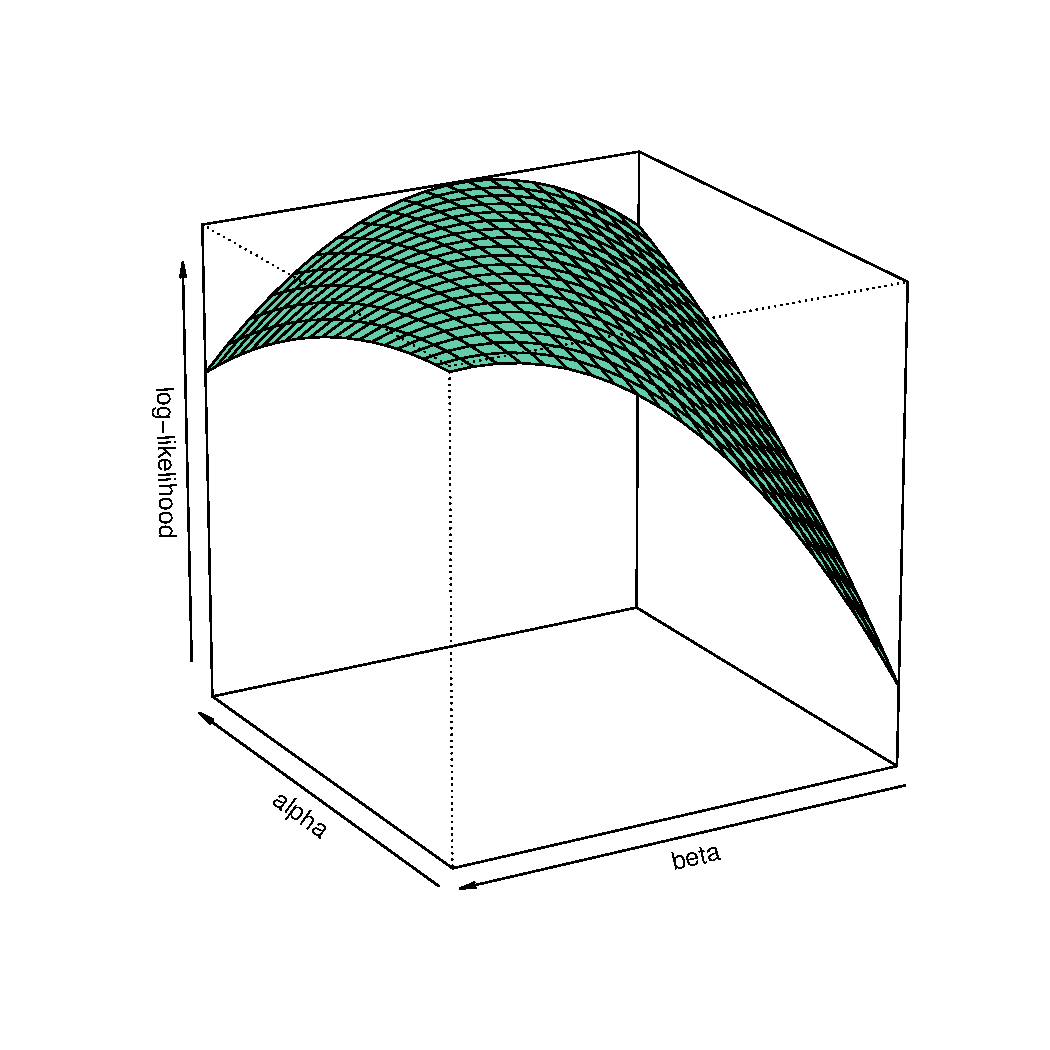
\includegraphics[scale=0.45]{pictures/week_24_ll_linear.pdf} 
\end{frame}

\frame{
\frametitle{Conclusion}
\begin{center}
All clear? More questions? \\
Thanks and see you next week!
\end{center}
}

\end{document}